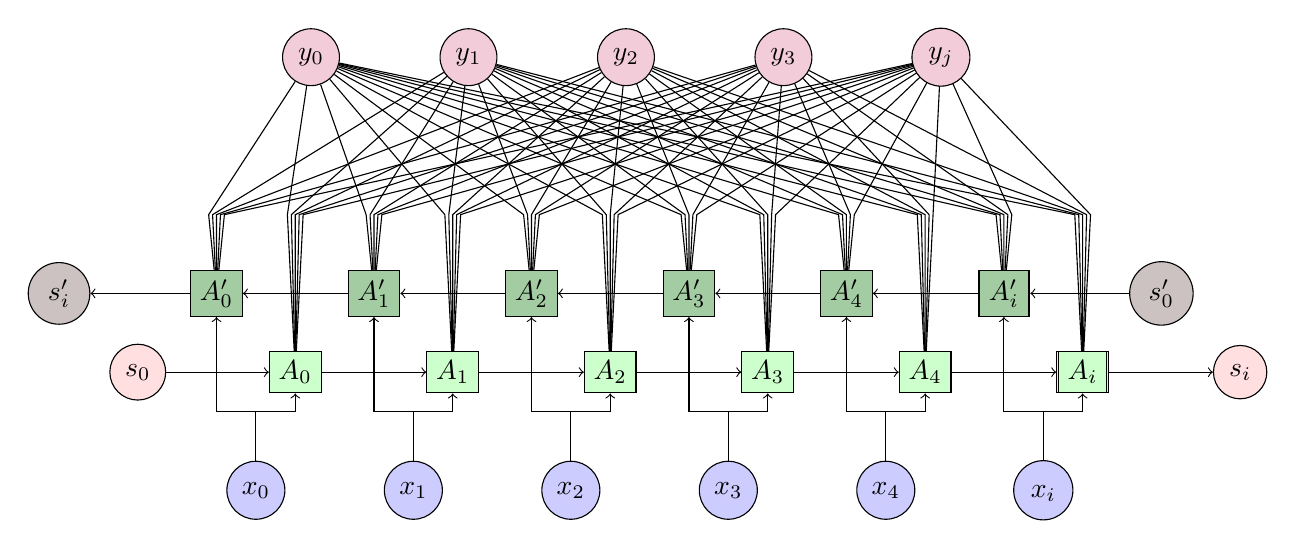
\begin{tikzpicture}
\foreach \i in {0,1,...,5} {
	\node[draw,fill=green!20] (f\i) at (\i*2,0) {$A_\i$};
	\node[draw,fill=green!20!white!80!black] (b\i) at ({(\i-0.5)*2},1) {$A^\prime_\i$};
	\node[draw,circle,fill=blue!20] (x\i) at ({(\i-0.25)*2},-1.5) {$x_\i$};
	%\node[draw,circle] (y\i) at ({(\i-0.25)*2},2.5) {$y_\i$};
	\draw[->] (x\i) -- +(0,1) -| (b\i);
	\draw[->] (x\i) -- +(0,1) -| (f\i);
	%\draw[->] (b\i) -- ++(0,0.5) -- ++(0.5,0) -- (y\i);
	%\draw[->] (f\i) -- ++(0,1.5) -- ++(-0.5,0) -- (y\i);
}
\node[draw,circle,fill=pink!50] (f-1) at (-2,0) {$s_0$};
\node[draw,circle,fill=pink!50] (f6) at (12,0) {$s_i$};
\node[draw,circle,fill=pink!20!white!80!black] (b6) at (11,1) {$s^\prime_0$};
\node[draw,circle,fill=pink!20!white!80!black] (b-1) at (-3,1) {$s^\prime_i$};
\foreach \i in {-1,0,1,...,4,5} {
	\pgfmathparse{int(\i+1)} % int is important
	\draw[->] (f\i) -- (f\pgfmathresult);
	\draw[->] (b\pgfmathresult) -- (b\i);
}
\foreach \j in {0,1,...,4} {
	\node[draw,circle,fill=purple!20] (y\j) at ({(\j+0.1)*2},4) {$y_\j$};
	\foreach \i in {0,...,5} {
		\draw (f\i) -- ++({-0.1+\j*0.05},2) -- (y\j);
		\draw (b\i) -- ++({-0.1+\j*0.05},1) -- (y\j);
	}
}
\node[draw,circle,fill=blue!20] at (9.5,-1.5) {$x_i$\vphantom{1}};
\node[draw,fill=green!20] at (10,0) {$A_i$\vphantom{1}};
\node[draw,fill=green!20!white!80!black] at (9,1) {$A^\prime_i$\vphantom{1}};
\node[draw,fill=purple!20,circle] at (8.2,4) {$y_j$};
\end{tikzpicture}